\documentclass{article}
\usepackage[utf8]{inputenc}

\usepackage{natbib}
\usepackage{graphicx}
\usepackage[margin=.75in]{geometry}
\usepackage{hyperref}
\usepackage{amsmath,amsthm,amsfonts,amssymb}
\usepackage{fancyhdr,multicol,enumerate}
\DeclareMathOperator{\spn}{span}
\let\oldhat\hat
\usepackage{wrapfig}
\renewcommand{\vec}[1]{\mathbf{#1}}
\renewcommand{\hat}[1]{\oldhat{\mathbf{#1}}}

\title{A Simple guide to text embedding with BERT for the first time}
\author{Savannah Amos, Yash Joshi, Drew Klaubert}
\date{June 2020}

\begin{document}

\maketitle

\section*{A few quick notes} 
\begin{itemize}
    \item This is a guide that will show how to use BERT to obtain embeddings of text.  We will cover everything from the initial installation of BERT, to showing how the model works and finally being able to embed our own pieces of text.
    \item This guide will be done using Anaconda and assumes that you already have it installed with some familiarity with it. It is also required that you are running a version of Python that is 3.5 or newer and have a fundamental understanding of the Python programming language.
    \item Mac Users Beware: This guide was done using a machine running windows and may not be completely compatible with the Mac operating system. Work-arounds for such issues are in development and will be supplied ASAP
    \item[]
    \textit{Optional: it is encouraged that you have some experience using word2vec before proceeding with this guide as that will build basic intuition as to how word embedding works}
\end{itemize}

\section*{Getting started(Installation)}
\begin{enumerate}
    \item \textbf{Tensorflow}:
    \begin{enumerate}
        \item[] We will require Tensorflow for this. From our experience, we will not be insalling the most recent version of Tensorflow as we have had some issues. Instead we will be using the most recent version of Tensorflow 1 which is 1.15.  This can be installed by entering the following command into the Anaconda prompt:
        
        \begin{center}
            \begin{verbatim}
                pip install --upgrade tensorflow==1.15
            \end{verbatim}
        \end{center}
    \end{enumerate}
    \item \textbf{Pytorch}
    \begin{enumerate}
        \item[] There are multiple ways to install and set up BERT. For the first part of this guide, we will be using the pytorch pretrained BERT model that is available from the people at Huggingface. The link to their repo is at the end of this document and we encourage you check it out. 
        You can install pytorch for your machine \href{https://pytorch.org/}{here}: \url{https://pytorch.org/}
    \end{enumerate}
    
    \item \textbf{BERT}
    \begin{enumerate}
        \item[] Now that we have other necessary thing, let's get BERT installed. This can be done with the following command in the Anaconda prompt:
        \begin{center}
            \begin{verbatim}
                pip install pytorch-pretrained-bert
            \end{verbatim}
        \end{center}
    \end{enumerate}
\end{enumerate}

\section*{Testing some basic features}
A lot of the information in this section is inspired by a notebook that was presented during an NLSea meetup in August of 2019.  This is the link to that githib repository \url{https://github.com/tobyatgithub/bert_tutorial}
\vspace{.25cm}\\
Before we get into looking at code, it is important to note the steps that are being taken by BERT to go from a word or sentence to an embedding. Starting with the sentence, we first need to tokenize it, then we will be able to change the tokens into IDs which will then be able to be put into the model so we can extract an embedding out of it. Those steps look like this:
\begin{center}
    words $\rightarrow$ tokens $\rightarrow$ IDs $\rightarrow$ hidden states $\rightarrow$ embedding
\end{center}


Now that we have done the necessary installations and intuition, let's start looking at some code that shows us how this thing can be loaded and used.

\begin{enumerate}
    \item To get this started, we need to load our necessary packages\\
    \vspace{.1cm}\\
        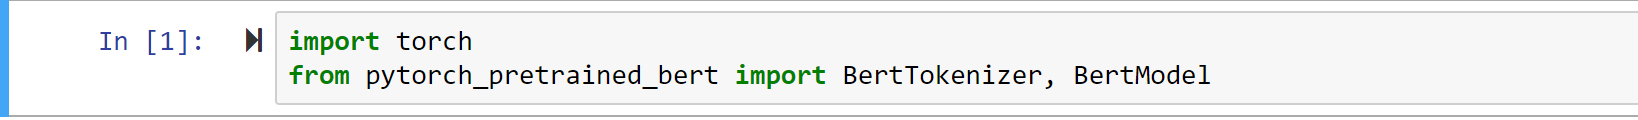
\includegraphics[scale = .8]{import2.png}
        \vspace{.2cm}\\
    \item Then we will load in the tokenizer which will be what turns our sentences into a sequence of tokens\\
    \vspace{.1cm}\\
    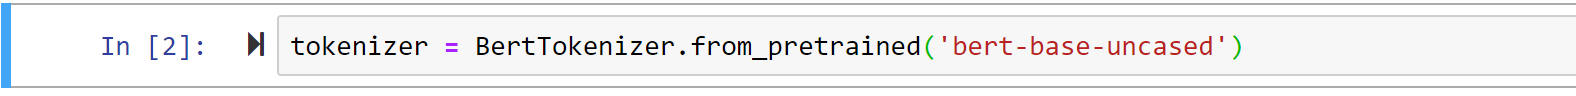
\includegraphics[scale = .8]{token_picuture2.png}
    \vspace{.2cm}\\
    
    
    \item For the tokenizer to work properly we need to add some tokens of our own.  One being "[CLS]" which marks the beginning of a text entry and the other being "[SEP]" which is the token that we put in between sentences within the same text entry.  So lets put together the following text.  "We are learning something very cool right now. Pay attention". After we put the tokens in the right places we get the following:\\
    \vspace{.1cm}\\
    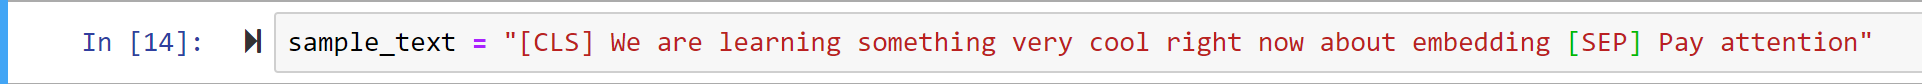
\includegraphics[scale = .7]{sample3.png}
    \vspace{.2cm}\\
    \item Now we can tokenize this sentence with the following code:\\
    \vspace{.1cm}\\
    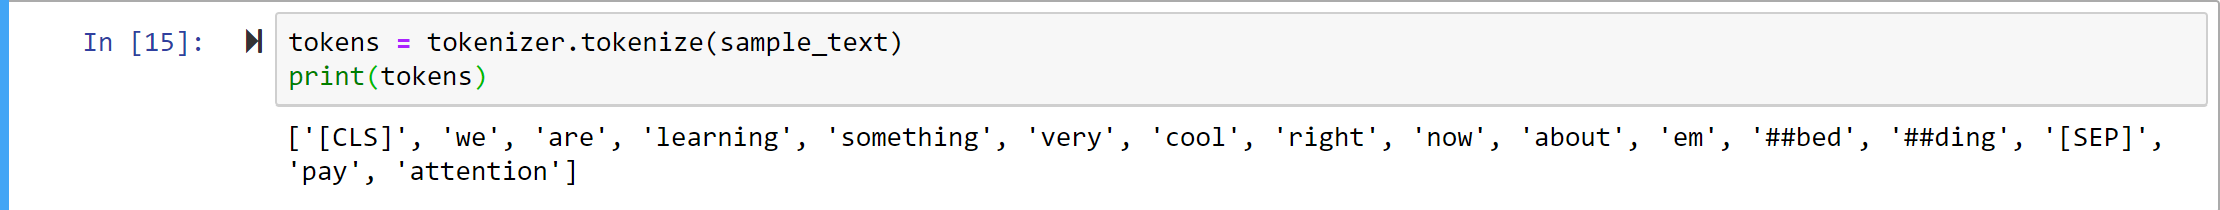
\includegraphics[scale = .6]{tokenstep2.png}\\
    \vspace{.1cm}\\
    Notice in this output that the word "embedding" is broken into 3 tokens.  A lot of words will do this especially root words that have prefixes or suffixes on them.
    \vspace{.2cm}\\
    \item We also want to keep in mind the space character that is separating the "[CLS]" and the "[SEP]" tokens from the text. Omitting the space between these tokens and the text is going to result in the following tokenization.\\
    \vspace{.1cm}\\
    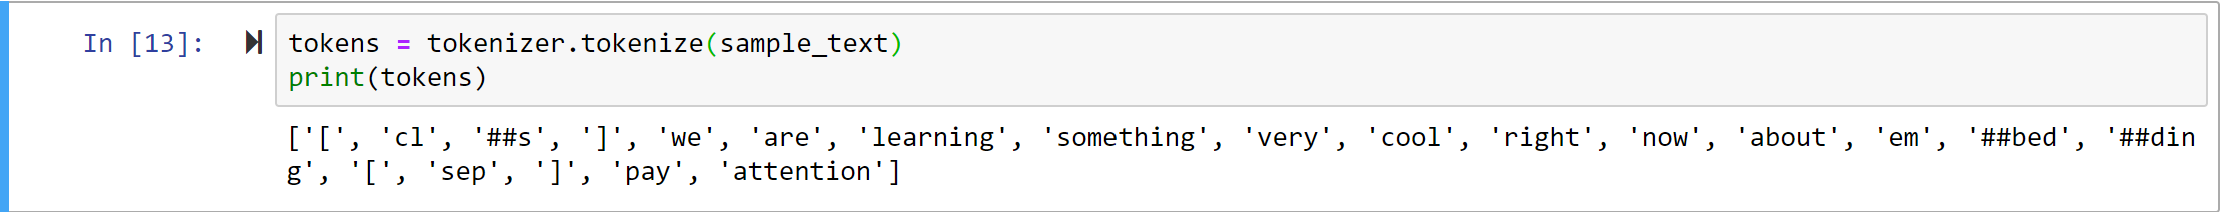
\includegraphics[scale = .6]{tokenstep1.png}\\
    \vspace{.1cm}\\
    In this output, we see that the CLS and SEP tokens themselves are being broken into multiple sections which is incorrect.
    
    \item Now we can get the token IDs that we will be feeding into the pretrained BERT model\\
    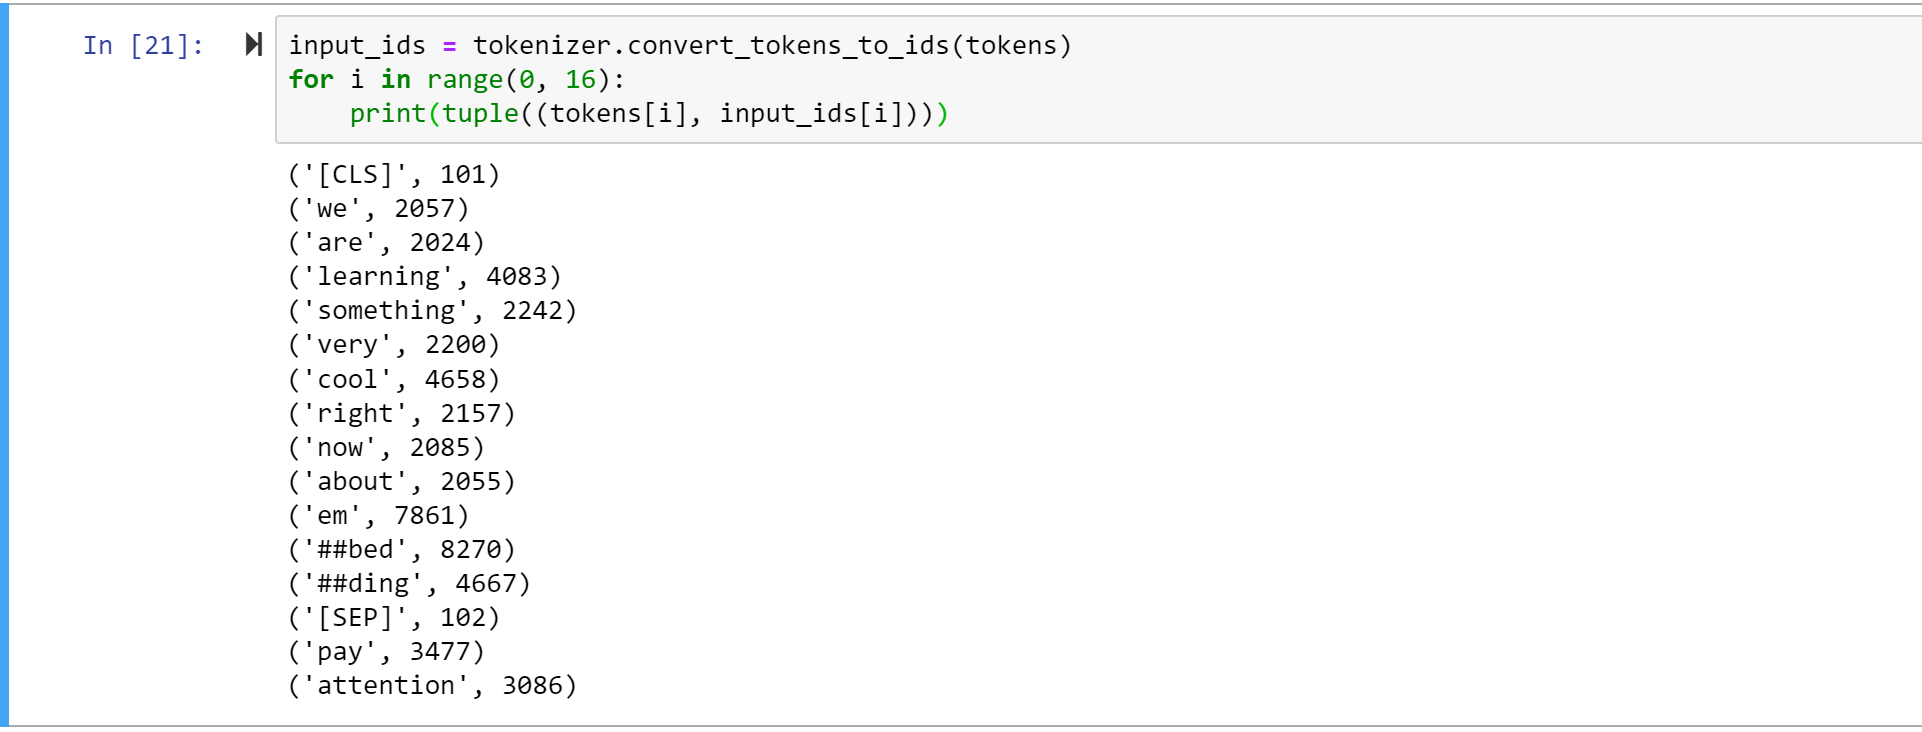
\includegraphics[scale = .7]{ids1.png}
    \vspace{.1cm}\\
    Now we have that each token has its own numerical ID
    
    \item The next step is to actually load the BERT model that the previous information can be put into this is done with the following code:\\
    \vspace{.1cm}\\
    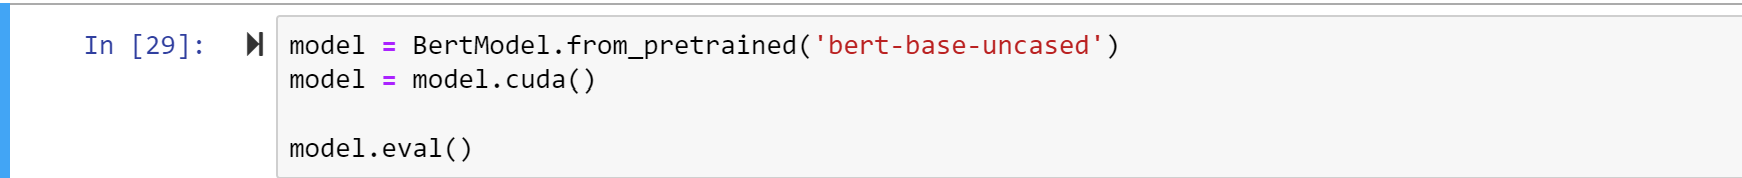
\includegraphics[scale = .7]{model_load.png}\\
    \vspace{.1cm}\\
    The first two lines are loading the version of the model that we are looking for.  We want the base, uncased model for this demonstration.  The third line is putting the model in evalutation mode.  You can explore the different versions of BERT in the official BERT github repository \url{https://github.com/google-research/bert}
    \vspace{.2cm}\\
    \item The next step is to go from the IDs to the hidden state vectors.  We will not go into too much detail as to how these are working so we recommend looking at some of the tutorials in the NLSea repository that is linked in the beginning of this section. In short the code to achieve this is:\\
    \vspace{.1cm}\\
    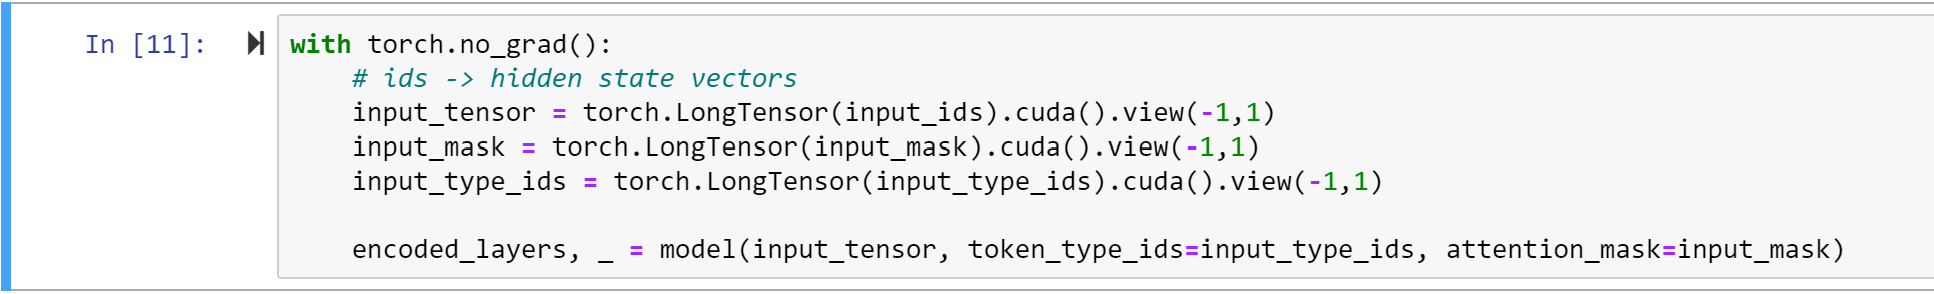
\includegraphics[scale = .7]{hidden.png}\\
    \vspace{.1cm}\\
    There are 12 embedding layers in the base model of BERT. We want to sum the vectors of the last 4 layers:\\
    \vspace{.1cm}\\
    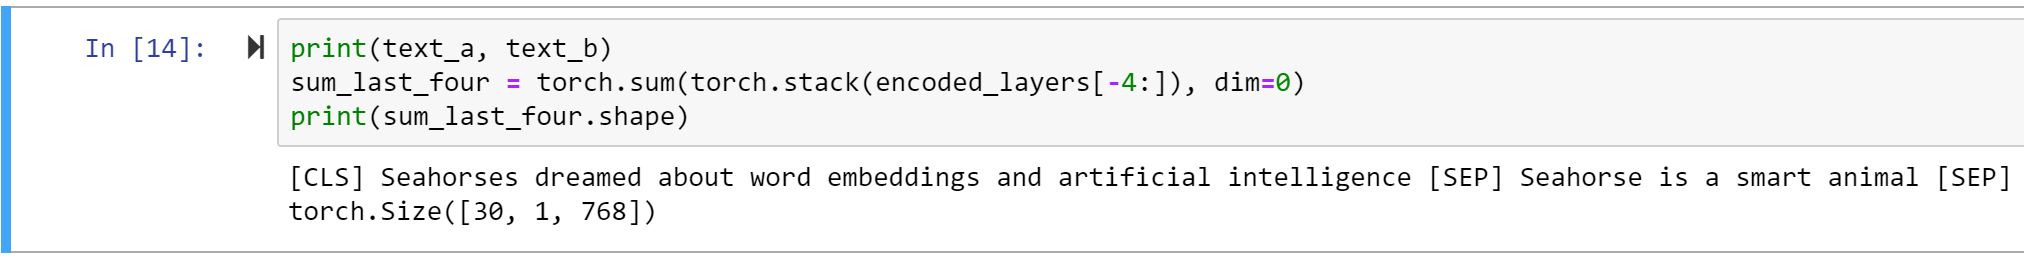
\includegraphics[scale = .67]{sum4.png}\\
    \vspace{.1cm}\\
    Note the shape of this object.  We have 30 different embeddings each of which are of 768 dimensions.  Each of these embeddings is representing a token in the original sentence that we used as an example.  So these are word embeddings. To get the entire sentence embedding, all we need to do is average out all of the 30 token embeddings:\\
    \vspace{.1cm}\\
    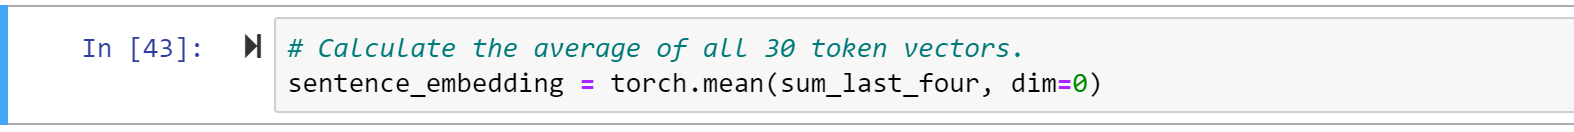
\includegraphics[scale = .8]{sentence_embed2.png}
    \vspace{.2cm}\\
    And there we have it! we have gone from a block of text all the way to an embedding.  In the next section we will be able to cut down on the amount of work needed to run this model.

\end{enumerate}

\section*{BERT-As-Service}

Now that we have the fundamental knowledge of how this model is working, lets use something that makes this process a little more repeatable. We will be using BERT-AS-Service.  Just like before, we will go through the process from installing to getting an embedding for a block of text.

\begin{enumerate}
    \item \textbf{Installation}
    \begin{enumerate}
        \item[] In order to use this, we need to install the BERT serving server and the BERT serving client. We can do that with the following few commands in the Anaconda prompt:
        \begin{center}
            \begin{verbatim}
                pip install bert-serving-server
                
                pip install bert-serving-client
            \end{verbatim}
        \end{center}
        \textit{Note: The requirements for the python and tensorflow versions remain the same as above.}
            \vspace{.2cm}\\
            We also need to make sure that we have a BERT model downloaded.  We are using the base uncased model for this demonstration which can be installed through the official BERT github repo linked above.
            
    \end{enumerate}
    
    
    \item \textbf{Running the Model}
    \begin{enumerate}
        \item[] Now that we have the installations done, all we need to do now is run the service.  This is done with the command:
            \begin{verbatim}
        bert-serving-start -model_dir [PATH TO MODEL] -num_worker=2 -max_seq_len 50
            \end{verbatim}
            
            \item[] You can change the number of workers and the sequence length as you see fit.  Make sure you have the exact path to where your BERT model is saved.  As an example, here is the command I used
            \begin{verbatim}
    bert-serving-start -model_dir uncased_L-12_H-768_A-12/ -num_worker=2 -max_seq_len 50
            \end{verbatim}
    \end{enumerate}
    
    \item \textbf{Using the client}
    \begin{enumerate}
    \item[] Now that we have the model running, all we need to do is call the service.  Here is what that code looks like:\\
    \vspace{.1cm}\\
    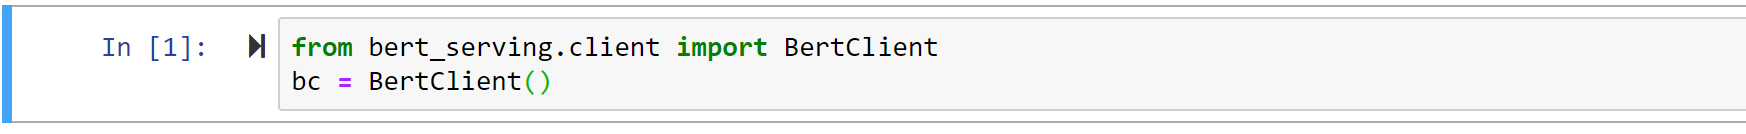
\includegraphics[scale = .7]{service_start.png}
    \vspace{.2cm}\\
    
    \item[] Then we can just simply get an embedding for the sample text block that we were working with in the last section:\\
    \vspace{.1cm}\\
    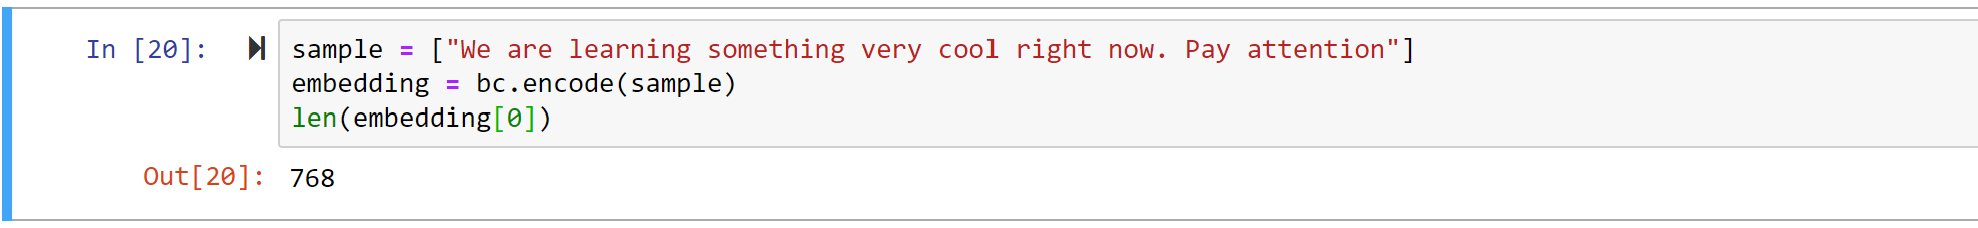
\includegraphics[scale = .625]{service_sample.png}
    
    \item[] And just like that we have a BERT embedding! We can also get separate embeddings for each sentence in this text block if we wish:\\
    \vspace{.1cm}\\
    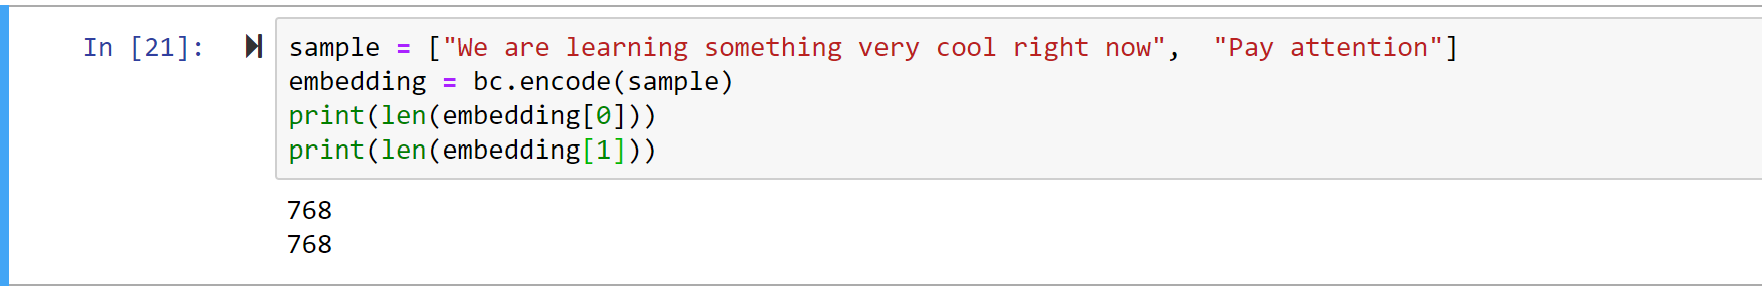
\includegraphics[scale = .7]{sample_list.png}\\
    \vspace{.1cm}\\
    Now we have two different embeddings. One for each of the sentences. Now we can start doing comparisons between these sentences through techniques like cosine similarity. In order to do that, we just need to import some libraries and conduct our experiment\\
    \vspace{.1cm}\\
    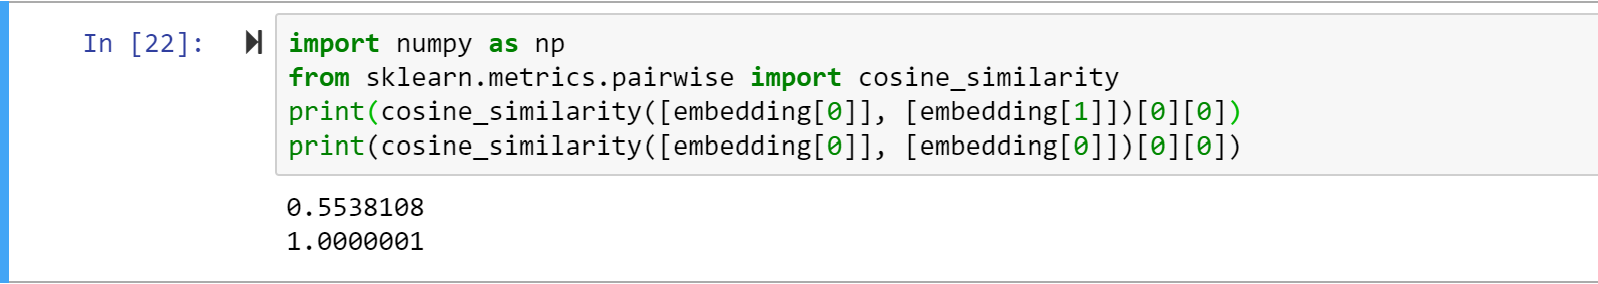
\includegraphics[scale = .775]{cosine_sim.png}
    \vspace{.1cm}\\
    Keeping in mind that cosine similarity will give us a number between 0 and 1, we see something that was to be expected. The similarity between the first and the second is not extremely high.  If we were to compare the first sentence to itself, we get the cosine of the angle is 1 so the angle itself is 0.\\
    \vspace{.2cm}\\
    A closing note on this: From our experiments we have found that embedding a sentence with BERT may be a little decieving.  Note in the first section, we took the embedding for all the tokens in a sentence and averaged them together.  Doing this tends to lose some of the context, especially when wanting to embed and entire paragraph.  The next section will address that issue.
    \end{enumerate}
    
    
\end{enumerate}

\section*{Sentence-BERT}

The past sections are great for embedding single words and some semantically simple sentences and will work great for most cases.  Embedding an entire paragraph may get a little tricky with those methods because we lose some of the context of the sentence by simply averaging all of the different word embeddings. This section will walk through Sentence-BERT which we have found to be a better way to embed an entire sentence in context.

\begin{enumerate}
    \item \textbf{Installation}
    \begin{enumerate}
    \item[]
    The installation for this is not too bad since we have a lot of the basic stuff already done. First we need to install sentence transformers which can be done with the following command in the Anaconda prompt:
    
    \begin{verbatim}
                        pip install -U sentence-transformers
    \end{verbatim}
    Note: You most likely already have this satisfied if you have done the two previous sections. 
    \item[] And that's it for the installation.  There is an alternative option for installation right through the UKPLab github repository that this portion of the guide is inspired from. They are liked below if you are interested in reading more. \\\url{https://github.com/UKPLab/sentence-transformers}
    
    \end{enumerate}
    
    \item \textbf{Using This Model}
    \begin{enumerate}
        \item[] Using this model is relatively simple to use and similar to using the Bert-as-service client. We need a cell in our python notebook the imports the sentence transformer:\\
        \vspace{.1cm}\\
        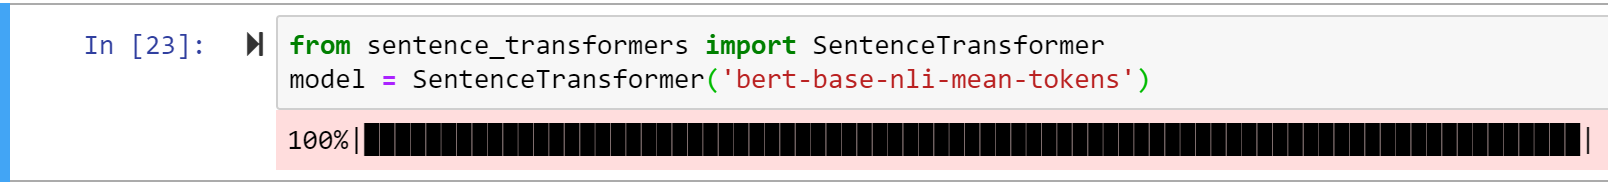
\includegraphics[scale = .77]{import_transform.png}
        \vspace{.1cm}\\
        Note: This took about a minute to fully download on my machine.
        
        \item[] Now we can simply start running our experiments like we were doing last time.  For this we will use the same sample sentences as before.\\
        \vspace{.1cm}\\
        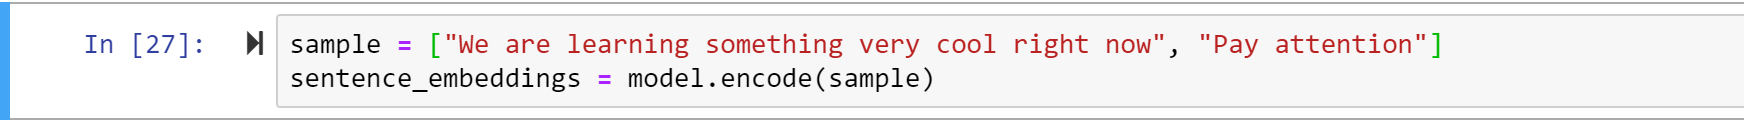
\includegraphics[scale = .71]{sentence_bert_example.png}
        \vspace{.1cm}\\
        And just like that we have embeddings of these sample sentences.  Now lets show that we get different embeddings with this version of BERT by doing another cosine similarity experiment.\\
        \vspace{.1cm}\\
        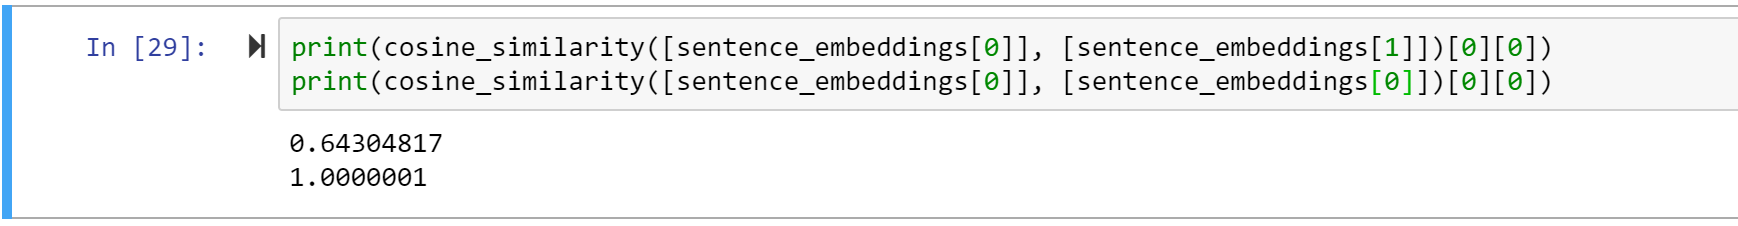
\includegraphics[scale = .715]{sentence_bert_cos.png}
        \vspace{.1cm}\\
        We are getting a different cosine similarity between the two sample sentences which means we are getting different embeddings.  Again, through our experimentation, this seems to be the best way to obtain embeddings for entire sentences and still be able to preserve the context of the sentence.
    \end{enumerate}
\end{enumerate} 

\section*{Conclusion}
So there is three different way of deploying BERT to get embeddings for words and sentences.  As stated before this guide is in the early stages of development and may have some flaws.  If any issues with this guide arise and are need of fixing, the emails to the contributors have been included below.

\begin{verbatim}
Savannah Amos - amos3@vt.edu
Yash Joshi - yashjoshi@vt.edu
Drew Klaubert - kdrew17@vt.edu
\end{verbatim}

\end{document}
